\documentclass[11pt,twoside,a4paper]{report}

\usepackage[utf8]{inputenc}
\usepackage{amsmath}
\usepackage{amsfonts}
\usepackage{amssymb}
\usepackage{url}
\usepackage{graphicx}
\usepackage{caption}
\usepackage{subcaption}
\usepackage{array}
\usepackage{booktabs}
\usepackage{listings}
\usepackage{color}
\usepackage{longtable}
\begin{document}

\definecolor{dkgreen}{rgb}{0,0.6,0}
\definecolor{gray}{rgb}{0.5,0.5,0.5}
\definecolor{mauve}{rgb}{0.58,0,0.82}

\lstset{
  language=Java,
  aboveskip=3mm,
  belowskip=3mm,
  showstringspaces=false,
  columns=flexible,
  basicstyle={\small\ttfamily},
  numbers=none,
  numberstyle=\tiny\color{gray},
  keywordstyle=\color{blue},
  commentstyle=\color{dkgreen},
  stringstyle=\color{mauve},
  breaklines=true,
  breakatwhitespace=true,
  tabsize=3
}
\title{Evaluation of algorithms for complex shielding in point kernel dose calculations}
\author{Tom Robert Bryntesen}
\date{May 2015}
\maketitle

\begin{abstract}
This thesis compares algorithms for finding the intersections with complex shields as part of the point-kernel algorithm. It is used to calculate a large number dose-rates, allowing dynamic visualisation of radiation fields and calculating doses in real time. This is used in training and planning work in environments containing radiation. The shielding calculations is the most time consuming part of the calculation when there is a complex environment. There is also a need to represent complex shapes that represent real world object. Three algorithms for calculating shielding have been implemented. One uses boolean operations on primitive shapes like boxes, cylinders and spheres to create complex objects. The second uses a triangulated geometry. The third uses a binary voxel grid. Each algorithm have been analysed and presented using the big O notation. The algorithms have also been benchmarked for performance, accuracy and memory usage. 

The voxel grid implementation have good running time characteristics. However the $O(n^3)$ memory usage limits the size of the grid and in turn the accuracy. The triangulated geometry method have $O(log(n))$ running time and low memory usage. However there is a problem with the algorithms that results in wrong output in certain rare situations. This may make in unsuitable for usage in dose calculations if they are used in making safety critical decisions. The boolean method with primitive shapes is the fastest method in the benchmarks. Using the boolean method on the sorted segments can also be extended to support other shapes than primitives, like voxels or triangulated geometry. This makes it a useful tool to have when making complex shielding.
\end{abstract}

\section{Acknowledgements}
I wish to thank my thesis supervisors Lars Magnusson at Østfold University College.

Ife

John Eidar Simensen

...

\tableofcontents

\chapter{Introduction}
In the nuclear field the workers are exposed to the risk of being exposed to radiation. In radiation protected the ALARA principle states that the risk shall be \textbf{A}s \textbf{L}ow \textbf{A}s \textbf{R}easonably \textbf{A}chievable. 

One way to lower the risk is to teach the workers about radiation. Software that visualise the radiation is helpful in that it lets the user see the radiation. Doing so can help teach about the factors in dose uptake. That is time of exposure, distance and shielding. When preparing for a job the worker can be briefed about the procedure by showing an animation with radiation visualisation \cite{szHoke2014comprehensive}. It is also possible to train on the procedure actively, in an interactive virtual reality environment. By seeing the areas with higher radiation levels the worker can take steps to avoid these, or minimise the time spent there in order to receive a lower dose. 

Another way to lower the risk is for better planning. Given a planning software that could estimate the doses of workers one could experiment to find the scenario that gives the lowest dose. Either by changing where the workers stand or putting up shielding.

This thesis will focus on improving the algorithm used to calculate dose-rates in real time. Specifically how to improve the performance of calculating the intersections with complex shields in the environment.

\section{Motivation}
In order to visualise radiation or calculate doses one need to do a great number of calculations. Many visualisation takes a 3 dimensional grid of values as input. If there are 20 cells in each dimension it would require 8000 measurements to generate the visualisation. If the scene is changing, for example when a shield or source is moving, the visualisation has to be updated at interactive rates. 

To calculate the dose of a worker over time one needs to integrate the dose-rate over time. For example the software would calculate the dose-rate for the worker every second and add it all up to get the dose. If the procedure last more than an hour thousands of calculations would be needed for each worker. To keep the software responsive the calculation need to be as fast as possible.

There are different ways to represent a radiological scene. If there are measurements in the area then interpolation can be used to estimate the value at an arbitrary position. However this would not allow for a dynamic scene where one can move sources or shields around. Another way is to define sources and shields and calculate the dose-rates from that. Monte carlo methods simulate photons radiating from the source threw the environment until it reaches the measuring position. This is accurate but very slow. The point-kernel method calculates the dose-rate by taking a single ray from the source to the measuring position and uses formulas and statistical data to estimate the dose-rate. This is not as accurate as monte carlo but is very fast. A more in-depth description of the calculation methods is given in chapter \ref{chapter:Background}.

One of the inputs to the point-kernel calculation is the how the ray intersects with the shields between the source and measuring position. This is the most time consuming part of the algorithm for a scene with many shields. By improving the performance of the shields calculation the software will run faster giving a better user experience. Or it would be possible to add more shields, increasing the realism and accuracy of the scene.
%[TODO: elaborate on other benifits]

This thesis is written in collaboration with Institute for Energy Technology (IFE). They have implemented a point-kernel calculator that is used in their software. It has support for simple shields like boxes and cylinders. They also support a complex shield that uses a triangulated mesh to represent arbitrary shapes. The evaluation of other ways to represent and calculate complex shield can help IFE improve their calculator.

\section{Research Objectives}
The work in this thesis will find alternative ways to represent complex shields. That is shapes that can be arbitrary and concave. Some of the alternatives will be selected and implemented. The implementations will be evaluated and compared. The following research questions will be focused on during the evaluation process:

\begin{itemize}
\item What algorithms exist that can be used to calculate intersection with complex shielding in a point kernel calculator
\item What are the algorithms performance characteristics
\begin{itemize}
\item Accuracy
\item Running time
\item Memory usage
\item Creation time
\end{itemize}
\item Are the trade-offs in the way the data to the algorithm are configured, for example between speed, memory and accuracy
\item How complex is the algorithm to implement
\item How practical is it to generate the data used as input to the algorithm
\end{itemize}


%\begin{itemize}
%\item How fast is the algorithm
%\begin{itemize}
%\item How does the shape of the shield influence the speed
%\end{itemize}
%\item How accurate is the algorithm
%\item How much memory does the algorithm use
%\item Are the trade-offs in the way the data to the algorithm are configured, for example between speed, memory and accuracy
%\item How complex is the algorithm to implement
%\item How practical is it to generate the data used as input to the algorithm
%\end{itemize}

\section{Scope and limitations}
The implemented software is intended to be used for benchmarking. It will not be integrated into existing dose calculation software. Doing so would require extra work and is not considered important in order to answer the research questions.

%When benchmarking the speed of the algorithms the initialisation of the algorithms are not included in the quantitative data. We will however discuss how the algorithms can be generated efficiently and if it can be pre calculated.

\section{Outline}
Chapter \ref{chapter:Background} gives an introduction to ionising radiation and methods of calculating doses. How the shield intersections are part of the calculation is explained. Examples of how it can be used in is presented.   A review of relevant ray tracing algorithms are presented.

Chapter \ref{chapter:Method} describes the methods used to evaluate the algorithms.

Chapter \ref{chapter:Design} explains the algorithms. Important implemenation details are presented. How the benchmarking is set up to generate the data needed for analysis is explained.

Chapter \ref{chapter:Results} shows the results of the algorithm analysis and benchmarks.

Chapter \ref{chapter:Discussion} discusses the findings produced in the Results chapter.

Chapter \ref{chapter:Conclusion} gives guidelines on when to use each algorithm, based on the findings from the test. Finally some recommendations for future work are offered.


\chapter{Background}
\label{chapter:Background}

%notes:
%In “Comprehensive support for nuclear decommissioning based on 3D simulation and advanced user interface technologies.” [4] page 375 it says “The investigations were performed using the Halden Planner (Figure 3) and VRdose (see Section 1) software, both of which are tools that offer real-time calculation (update) of personal and collective dose, dose rates and dose history (dose charts) while allowing the user to dynamically modify work scenarios. This greatly facilitates identifying optimal worker routes, shielding configuration, order of subtasks, and so forth by enabling suboptimal solutions to be quickly rejected. Furthermore, real-time visualisation of radiation risks (dose) [13,14] aids users in understanding the radiological conditions and, thus in determining the best directions for refining a work scenario during the optimisation process.”. In results: “Our investigations show that dynamic (real-time) tools that produce reasonably accurate radiological risk estimation can provide vital input information for decision-making, such as to be able to make an informed choice between remote-controlled and manual techniques for a decommissioning task.”

CAD-BASED MODELING FOR 3D PARTICLE TRANSPORT \cite{wu2009cad}. "bi-directional conversion between commercial CAD systems and the neutron transport simulation codes and the visualization of mixed rendering of geometry model and 3D volume data."

\section{Radiation Theory}
Ionising radiation. Alpha, beta, gamma. Focus on gamma since other can be shielded by clothing, gamma can go threw materials of long distances. Energies. How it is absorbed by the body and how it damages the body and dna. Cover distance, shielding and time.

\section{Usage in computing}
More general usage.

\subsection{applications}
Halden planner and Sim Editor. Other applications,

\section{Particle transport simulation using Monte Carlo method}

Particle transport simulation calculates radiation by simulating the radiation particles from the sources to the measurement position. It uses the Monte Carlo method \cite{wiki:monte_carlo_method} is used to determine how the particles interact with the surrounding matter.




Particle transport simulation

[3] explains an monte carlo implementation its methods. Too complex to get into in details. But basicly a large number of particles are simulated from source. The amount and energy reaching the receptor determines the dose.

Monte Carlo code MCBEND

"MCNP is a general-purpose Monte Carlo N-Particle code that can be used for neutron, photon, electron, or coupled neutron/photon/electron transport. Specific areas of application include, but are not limited to, radiation protection and dosimetry, radiation shielding, radiography, medical physics, nuclear criticality safety, Detector Design and analysis, nuclear oil well logging, Accelerator target design, Fission and fusion reactor design, decontamination and decommissioning. The code treats an arbitrary three-dimensional configuration of materials in geometric cells bounded by first- and second-degree surfaces and fourth-degree elliptical tori."
https://mcnp.lanl.gov/

MCNP has existed as MCNP since the mid 1970’s.
Initial geometry capability was Constructive Solid Geometry (CSG)
Macrobody capability was added (1980’s) where the macrobody
surfaces were translated into CSG surfaces.
%https://laws.lanl.gov/vhosts/mcnp.lanl.gov/pdf_files/la-ur-14-25120.pdf

\section{Point-kernel}
Reference Iztvans paper. Show function and explain part containing shielding.
matter and ways to determine results. TODO: try to find some overview/review paper.

Explain how shielding fits into the point kernel equation and that raytracing can be used to find data data needed.

Chucas \cite{chucas2000streaming}

\section{Raytracing}
Raytracing is used to determine distance travelled through shielding. Different ways to represent 
\subsection{Voxels}
fdsf
\subsection{Triangles}
fasdf
\subsection{Primitives}
fdfs
\subsection{Boolean}
df


\chapter{Method}
\label{chapter:Method}
This chapter describes how the algorithms will be analysed. The worst and average case complexity will be represented by big O notation is covered in section \ref{section:Analysis_of_algorithms}. The algorithms will also be tested empirically using benchmarking and is discussed in section \ref{section:Benchmarking}.

\section{Design and implementation}
Should we talk about development methodology. Iterative, unit tests, version control etc?

\section{How to evaluate algorithms}
Overview, analysis, benchmarking and profiling.

\section{Analysis of algorithms}
\label{section:Analysis_of_algorithms}
The complexity of an algorithm is often expressed using big O notation.
Upper and lower bounds are usually stated using the big O notation, which hides constant factors and smaller terms. Interested in worst and average case

Can not be compared because n represents different things.


%http://en.wikipedia.org/wiki/Computational_complexity_theory
%http://en.wikipedia.org/wiki/Analysis_of_algorithms

Discuss advantages and shortcommings of emperical (measured data) and analysis.

“Empirical evidence (also empirical data, sense experience, empirical knowledge, or the a posteriori) is a source of knowledge acquired by means of observation or experimentation.”

\subsection{Running time}
How is running time analysed.

\subsection{Memory usage}
Discuss data structure and how it fits with big O.

\subsection{Correctness}
Are there anyway to analyse this? Probably not but we can mention something here.

\section{Benchmarking}
\label{section:Benchmarking}

\subsection{Measurements}
Measure time used to run the algorithms against a chosen dataset.

Measure memory used to create and run algorithms against datasets.

\subsection{Datasets}
What methodology is used in choosing datasets. Realistic, find how it scales, can be compared with big O analysis.

\subsection{Data Collection}
An automatic benchmarking framework was created to be able to rerun the tests automatically. Benchmarks data set was created to be similar to real world usage. The output of the benchmarks are data that can be easily imported into analysis tools.

\subsection{Data analysis}
The benchmarking framework produces quantitative measurement for running time and correctness. This data will be analysed for comparing the algorithms. The experience from implementing the algorithms will also be reported on.

\section{Could do profiling of the code}
Have to find a method for that. Probably delete this part.


\chapter{Design, Planning and Implementation}
\label{chapter:Design}
This chapter describes how the project was designed in order to answer the research questions. Section \ref{section:Algorithms} explains the algorithms and covers the most important parts of the implementation. Section \ref{section:Design_Benchmarking} describes how the algorithms are benchmarked. This includes how the measures are collected and what test data to use.

\section{Algorithms}
\label{section:Algorithms}
This sections describes the algorithms and the most important implementation details. 

\subsection{Closed Mesh}
The closed mesh algorithm determines the intersection with the shield by intersecting the segment against the triangles in a mesh. The algorithm first finds all intersections between an infinite ray starting at the source position in the direction of the measurement position. If the start point is inside or outside the shield is determined by counting the number of intersections. It is inside if there are an odd number and outside if there are an even number of intersections. Then the intersections are iterated in sorted order from the source. Stopping when reaching the measurement positions or when there are no intersections left. Intersections are found when intersecting triangles and keeping track of if the ray is inside the mesh or not.

For the algorithm to work there need to be a way to determine if the source position is inside or outside the shield. This can be done if the mesh is closed, that is creating watertight surface that does not self intersect. One can count the number of intersections using an infinite ray starting from the source position. The ray can go in any direction but using the direction to the measurement positions one can reuse the intersection calculations. If the ray intersects an odd number of times the source position is inside.

%http://en.wikipedia.org/wiki/Even%E2%80%93odd_rule
%http://en.wikipedia.org/wiki/Point_in_polygon

TODO: image explaining algorithm,

\subsection{Bounding Volume Hierarchy Mesh}
The bounding volume hierarchy (BVH) mesh shield is an optimised version of the closed mesh. The difference is that the triangles are put in a bounding volume hierarchy of axis aligned bounding boxes (AABBs). The assumption is that this will perform significantly faster. At least for meshes with many triangles. Although at the expense of initialisation time and possible memory.

TODO: image visualising a BVH, how the BVH is created and that it is a $O(n^3)$ algorithm.

\subsection{Boolean Shape}
The boolean shape is build from primitives and are combined using boolean operations. For this benchmark we have limited the number primitives to boxes, spheres and cylinders. The boolean operations are limited to \textbf{or} and \textbf{subtract} operations. The or operations combines a list of children. The subtract operation subtracts one child from another. A child can be a primitive or another boolean operation.

To find the intersections the tree structure formed by the boolean operations and primitives are traversed. The return value of a node in the tree is a sorted list of intersecting line segments. For the primitives this will be where the line segment entered and exited it. For the \textbf{or} boolean operations this will be all the segments of the children merged so that there is no overlapping segments. For the \textbf{subtract} operation this will be all the segments in the second child removed from the segments of the first child.

The returned segments are represented as two values representing the segment endpoint. Each endpoint is represented by an “t” interpolator value from the source position to the measurement position. This way the boolean operations can be performed on 1 dimensional segments, which simplifies the implementation.

position = sourcePosition + t * (measurementPosition - sourcePosition)

TODO: implementation details

\subsection{Voxel Grid}
The voxel grid is a three dimensional grid where each cell represents whether or not the space of the cell is part of the shield. A fast voxel traversal algorithm \cite{amanatides1987fast} is implemented. The source code can be found in appindex \ref{source:Voxel_Grid_Raytrace}. The idea is to compute the t values of the next subdivision planes along each axis and choose the smallest one in every iteration to determine the direction for the next step.

The source code in figure \ref{fig:voxel_step} show the incremental part of the algorithm in 2 dimensions. 
\begin{itemize}
\item t is the interpolator along the line segment where 0 is at the start and 1 is at the end
\item tNextX and tNextY is the value of t when the ray will intersect the next edge of the voxel of the respective axis
\item dtDx and dtDy is how far t have to increase for going from one edge to next of the respective axis
\item xInc and yInc is either 1 or -1 and specifies which direction the ray is travelling along the respective axis
\end{itemize}
\begin{figure}[h]
    \centering
\begin{lstlisting}
    private void step() {
        if (tNextX < tNextY) {
            x += xInc;
            t = tNextX;
            tNextX += dtDx;
        } else {
            y += yInc;
            t = tNextY;
            tNextY += dtDy;
        }
    }
}
\end{lstlisting}
    \caption{Voxel step method}
	\label{fig:voxel_step}
\end{figure}

The algorithm chooses which axis that will hit an edge first. It stores the time of intersection in t. The index of the current voxel (x or y) and when it will hit the next edge (tNextX or tNextY) of the chosen axis is updated. 

The step method will be called in a loop. The loop will end when t is larger than 1 meaning it has passed the endpoint of the segment. It will also end if it has stepped outside the grid bounds. The loop also keeps track of when the ray enters and exits shielding cells and outputs intersections when appropriate.

The initialisation part of the algorithm consist of finding the variables used in the step method. If they ray starts outside the grid the intersection have to be found and the adjacent voxel have to be used as starting point. 

\section{Benchmarking}
\label{section:Design_Benchmarking}

\subsection{Java}
Java \cite{wiki:java} was chosen as the programming language used to implement the algorithms. Java is general-purpose object-oriented language. The source code is compiled into bytecode that can run on a Java virtual machine (JVM). That makes it possible platform independent and can run on any system that have implemented a JVM. 

The main reason for choosing Java is that it is the language used at the Halden Virtual Reality Center \cite{site:hvrc} at IFE. Using Java will make it easier to integrate the code into the existing software. The author has also experience in writing optimised code in this language.

\subsection{Threading}
One way to make an algorithm run faster on modern hardware is to use threading to run parts of the calculations in parallel. This is becoming increasingly important on modern CPUs as the main increase in speed comes from increased number of cores instead of increasing the clock frequency. For an implementation of a point kernel calculator it would make sense to thread out the calculations at the ray level. That is each ray, or group of rays, run in chunks. Therefore the shield intersection algorithms have not been implemented to use threading internally. However they have been written to be thread safe. They have to be able to be invoked safely from multiple threads at the same time. 

This has implications on how temporary data and calculations are stored. There are several ways to do this in Java. New objects can be created on the fly when needed. This is slow when done in performance critical sections of the code. Even though the garbage collector has become faster there is still an overhead in creating, initialising and collecting objects. An other way to create thread safe code is to synchronise sections of code that use shared data. This is also slow since threads can not work on the same code simultaneously. Forcing them to wait on each other. Also the synchronising mechanism in Java is relatively slow. The method chosen instead is to use ThreadLocal. This is the same as using static variables, however each thread get its own instance so it is thread safe. It is also fast.

\subsection{framework}
For the voxel implementation an analysis of the relationship between number of divisions and the results was performed. For comparisons with the other algorithms the error data was used to select the lowest division that resulted in an error \% lower than 1. For the tube and sphere shapes the lowest subdivision resulting in an error \% lower than 1 was selected for comparison.

A benchmarking framework was created to produce the quantitative data. The goal of the framework was to simplify the collection of and to produce unbiased data. The framework was designed to run all tests without the need of any human interaction. This made it easy to rerun the tests if any changes was made to the algorithms. It also made it easy to run the tests repeatedly and generating more reliable results by basing the data on a larger data set.

TODO: the rest is probably to detailed. Needs to be rewritten

The benchmarking framework will have a function that benchmarks a shape against a set of segments:

static BenchmarkOutput doBenchmark(String name, Supplier<ComplexShield> shieldCreator, List<Segment> segments, float[] correctTotals)

The name is used to identify the test and is returned in the BenchmarkOutput. 

The shieldCreator creates a shield. All the data must be created in the Suppler.get() method to be able to measure how much memory the shield uses.

The segments are all the line segments to test against the shield. The different algorithms will be tested against the same set of segments.

The correctTotals array contains what is considered to be the correct result for each segment. This is used to calculate the error the tested shield.

The memory, performance and correctness results are stored in BenchmarkOutput. This is the raw data from the benchmarks. The BenchmarkOutput is gathered, processed and written to a file. The file is imported into an external tool that can generate graphs.

A benchmarking class is created that sets up and performs the benchmarking for all the shapes. For each shape it will create a new set of segments. This is because the size of the shapes may vary and the segments must be adjusted accordingly. It will also implement the shieldCreator for each algorithm as well as calculating the correct results for the shape. 

\subsection{Measure memory used}
To calculate the amount of memory used by a shield we will log the memory used by the Java Virtual Machine (JVM) before and after creating an implementation. This will measure the memory needed to hold the data structures used to represent the shield. The JVM uses a heap to store all the data of the application. It has methods for querying the total amount of memory and approximate amount of free memory in the heap. By subtracting the free memory from the total we get approximately how much memory is used. However the JVM uses a garbage collector to collect memory that is no longer in use. Since the free memory reported do not include garbage not collected yet, the calculated memory used is not exact. To help we ask the JVM to perform garbage collection before calculating the memory used. But the documentation states that this is only a suggestion and it may not collect all garbage at this request. That this measure can be inaccurate must be taken into consideration when analysing the results. 

\subsection{Running time}
To measure running time the the high accuracy timer provided by the Java Virtual Machine is used. How the JVM calculates the time is not documented and may vary depending on operating system and hardware. The resolution of the timer was instead measured on the machine performing the benchmarks. This was done by calling the timer in a loop and logging the difference in value when it changed. See appendix \ref{source:timer_timer_resolution} for the source code. The resolution calculated on the test machine was 292 nanoseconds. This was considered to be more than enough for measuring the running time of the shielding calculations.

\subsection{Correctness}
The correctness is included in the benchmarking because the algorithms can not, in some cases, represent the real shape of the shield perfectly. Round shapes have to be approximated by for example triangle or voxel representations. There can also be a trade-off between correctness on one side and running speed and memory usage on the other. A voxel representation can use more cells to get more correct results at the expense of longer traversal times and higher memory usage. 

To determine the correctness of an algorithm it must be compared to what is considered to be correct. Boolean shields will be used as the correct representation for the shapes benchmarked in this thesis. This is because it is the only algorithm that can represent round shapes like spheres and cylinders correctly. Other types of shapes that are not supported by the boolean implementation will not be used in the benchmarks because of the need of having a correct representation.

The correctness is calculated as the sum of the error for each segment. The error for one segment is the absolute difference between the correct and calculated distance travelled. The error percentage is calculated using the correct sum and the sum of errors.

\subsection{Test Data}
The test data for the benchmark includes a set of shapes and the segments that will be tested against the shapes. The shapes are chosen for different reasons. The shape can be realistic, a shape that can be encountered in a real situation. Or it can be stylised, designed to answer a specific research question or a specific performance situation. The segments are designed to be a realistic example of how it would be used in an application.

\subsubsection{Segments}
The segments used in the benchmark are created to mimic that used in a application that visualise radiation. It will have a set of point sources and a set of measurement positions. A segment is created from each point source to every measurement position.  

The measurement positions will created as a 3 dimensional grid that is slightly larger than the bounding box of the shape. The size of each cell is set to the largest dimension of the grid divided by 30. That will give a grid of approximately 10000 measurement positions, given the axis of the bounding box have about the same length. 10 random points inside the bounding box is used to represent the point point sources. 

\subsubsection{Tub shape}
\begin{figure}[h]
    \centering
    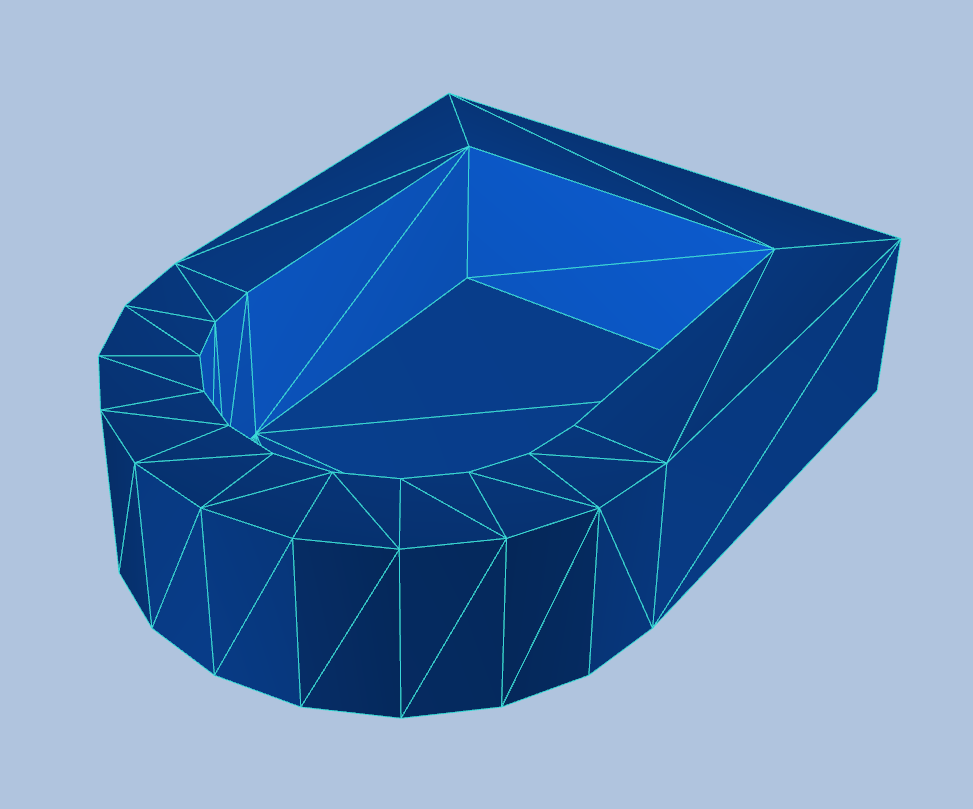
\includegraphics[width=0.45\linewidth]{images/tub_mesh}
    \caption{Tub shape}
    \label{fig:Tub shape}
\end{figure}

The tub shape was chosen because it is a realistic example of a complex shield. A customer of IFE needed to model this shape in the Halden Planner software. At the time there were no support for complex shields. It is one of the concrete reasons why the research into modelling complex shields were started. The shape consist of tub where one side is square and the other is round.

\subsubsection{Building shape}
\begin{figure}[h]
    \centering
    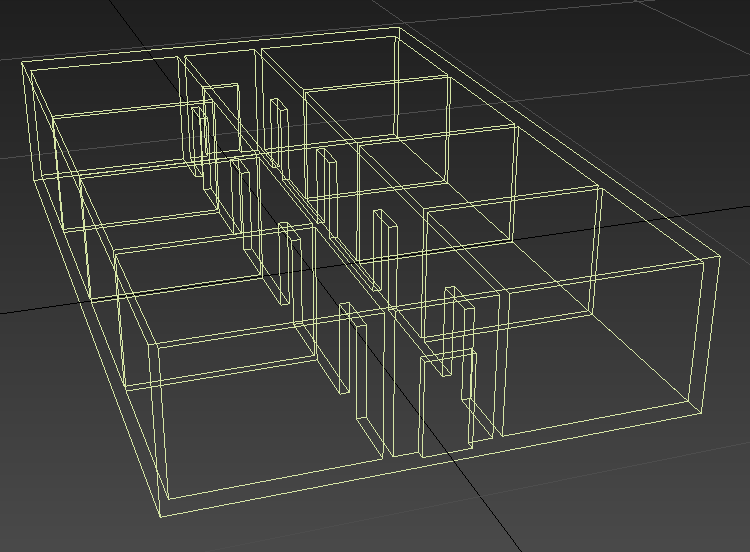
\includegraphics[width=0.45\linewidth]{images/room_max}
    \caption{Building shape}
    \label{fig:Building shape}
\end{figure}
In a radiological scene the building itself can be a major part of the shielding. To test this scenario a floor of a building was modelled. It consist of 8 rooms connected by a hallway. There is a door to each room as well as 2 doors entering the hallway.

\subsubsection{Box shape}
The box shape was included to see how well the complex shields are able to handle simple shapes. The box shape is one of the most useful shapes when building up a realistic radiological scene. If the complex shield handles it well then there might not be need for the application to have specific simple shapes, which can simplify the application. To make the scenario more complex the box is rotated 20, 30 and 40 degrees around the x, y and z axis respectively.

\subsubsection{Sphere shape}
The sphere shape was included to determine how the algorithms manages to represent a round shape. What are the speed, accuracy and memory trade-offs depending on how tessellated the mesh is or how many cells are used. 

\subsubsection{Tube shape}
\begin{figure}[h]
    \centering
    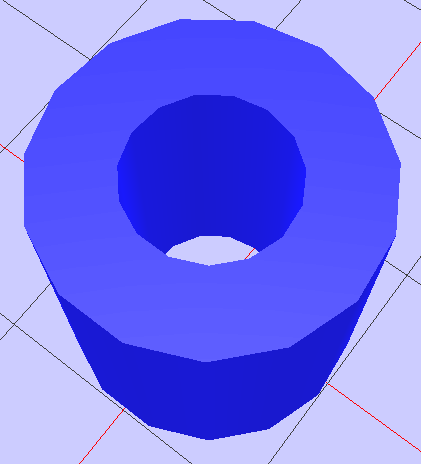
\includegraphics[width=0.45\linewidth]{images/tube_mesh}
    \caption{Tube shape}
    \label{fig:Tube shape}
\end{figure}

The tube shape was included because it is a round shape and it is realistic. There are many shapes in a nuclear power plant that that can be represented by a tube. For example waste containers and pipes.



\chapter{Results}
\label{chapter:Results}
%Outcome of the actual research work described in the implementation.
Section \ref{section:results_big_O} presents the big O analysis of the algorithms. Section \ref{section:results_benchmarking} presents the results of the benchmarking outlined in the benchmark design section \ref{section:Design_Benchmarking}.



%What can be mentioned: data quality, size of dataset, 

%Dimensions: 
%-algorithms (mesh, bvh, voxel, bool)
%-measures (running time, creation time, memory, correctness)
%-analysis methods
%  -analysis
%  -benchmarking
%    -shapes (box, sphere)

\section{Big O analysis}
\label{section:results_big_O}

\subsection{Boolean}
The boolean algorithm uses a tree data structure. Leaf nodes are primitives in our case, but can be anything that can be intersected with a line segment and return a sorted list of intersections. The internal nodes are boolean operations as subtract, unite or intersect. The whole tree has to be traversed to find the correct results. That is an $O(n)$ operation. However the internal nodes 
    
\subsection{Voxel}
In the voxel algorithm the cells in the grid is walked along the ray. Here n is the number of cells along the axis of the grid. Even though the three axis can have different number of cells we use n to represent all axis in the big O notation. The worst case and average complexity of the running time is is O(n). The memory needed to store the grid is one bit for each cell. The memory complexity is O($n^3$).


\subsection{Brute force triangles}
For the brute force triangle intersection algorithm the main part of the algorithm is to check each triangle against for intersection with the ray. The running time complexity is O(n) given n is the number of triangles. This is true for the best, average and worst case. The memory complexity is also O(n) given n is the number of triangles.

\subsection{Bounding Volume Hierarchy triangles}
For the BVH implementation of the triangle intersection algorithm the complexity depends on the depth of the tree. The tree generation algorithm implemented for this paper do not guarantee a fully balanced tree. So the worst case running time is $O(n)$. However it creates a fairly optimal tree which on most cases is relatively balanced. So the average running time is $O(log n)$. The number of internal nodes in a binary tree is roughly the same as the leaf nodes. So memory complexity for the BVH tree implementation is O(n). This holds for both worst and average case.

\subsection{Summary}
Table \ref{tab:big_o_summary} gives an overview of the worst and average case running time complexity. It also shows the memory complexity of the algorithms.

\begin{table}[htbp]
  \centering
  \caption{Complexity of algorithms}
    \begin{tabular}{rrrr}
    \toprule
    Algorithm & Worst case & Average case & Memory complexity \\
    \midrule
    Boolean & $O(n)$ & $O(n)$ & $O(n)$ \\
    Voxel & $O(n)$ & $O(n)$ & $O(n^3)$ \\
    Brute force triangles  & $O(n)$ & $O(n)$ & $O(n)$ \\
    BVH triangles  & $O(n)$ & $O(log n)$ & $O(n)$ \\
    \bottomrule
    \end{tabular}%
  \label{tab:big_o_summary}%
\end{table}%

All algorithm have $O(n)$ worst case running time complexity. All algorithms also have $O(n)$ average running time as well, except for the BVH triangles which have $O(log n)$. This makes the algorithm that scales the best with regards to running time. The memory complexity is $O(n)$ for all algorithms except for Voxel which have $O(n^3)$. This severely limits the size of the grids that can be used.



\section{Benchmarking}
\label{section:results_benchmarking}

\subsection{Voxel grid}
\begin{figure}[h] \centering 
	\begin{subfigure}[h]{0.49\textwidth} 
	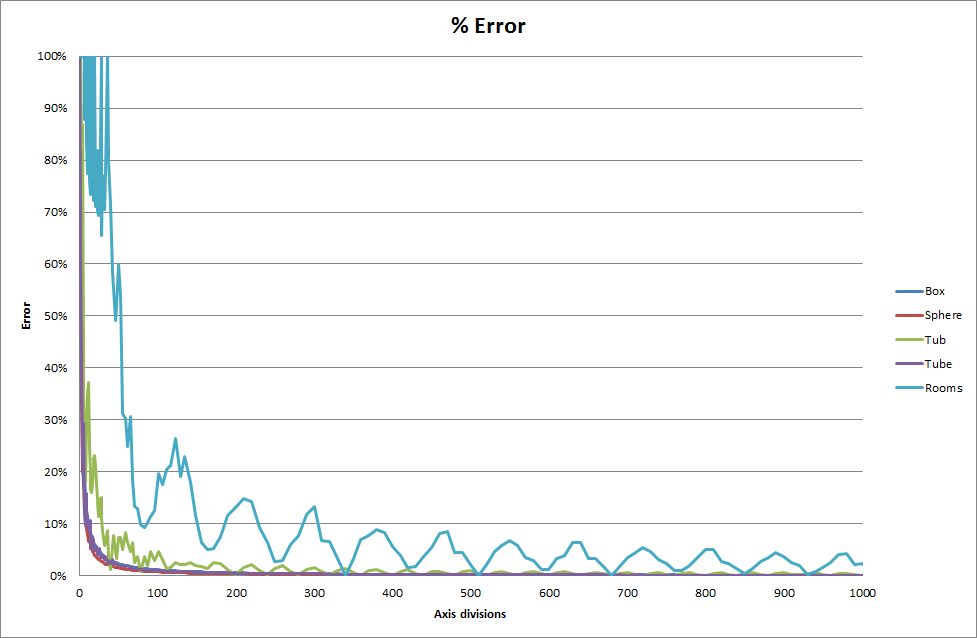
\includegraphics[width=\textwidth]{images/chart_voxel_error}
	\caption{error} \label{fig:voxel error} \end{subfigure}
    \begin{subfigure}[h]{0.49\textwidth}
	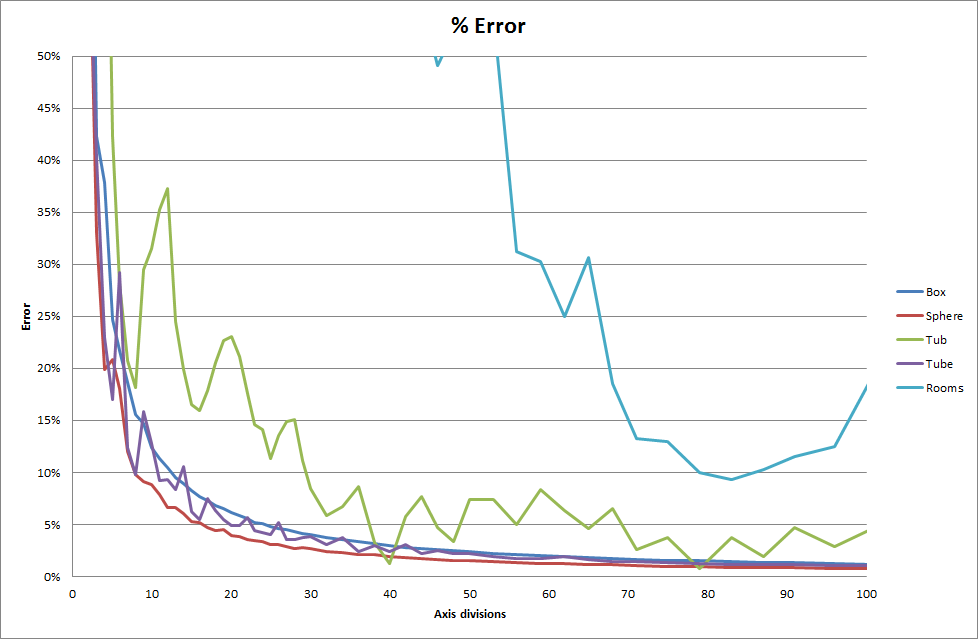
\includegraphics[width=\textwidth]{images/chart_voxel_error_zoomed}
    \caption{error zoomed} \label{fig:voxel error zoomed} \end{subfigure}
    \begin{subfigure}[h]{0.49\textwidth}
	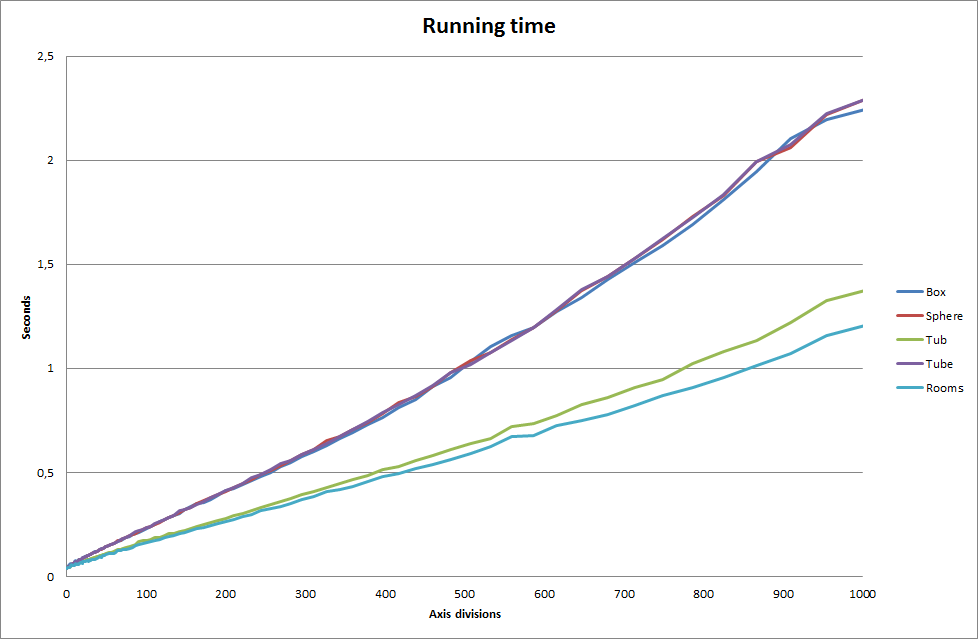
\includegraphics[width=\textwidth]{images/chart_voxel_running_time}
    \caption{running time} \label{fig:voxel running time} \end{subfigure}
    \begin{subfigure}[h]{0.49\textwidth}
	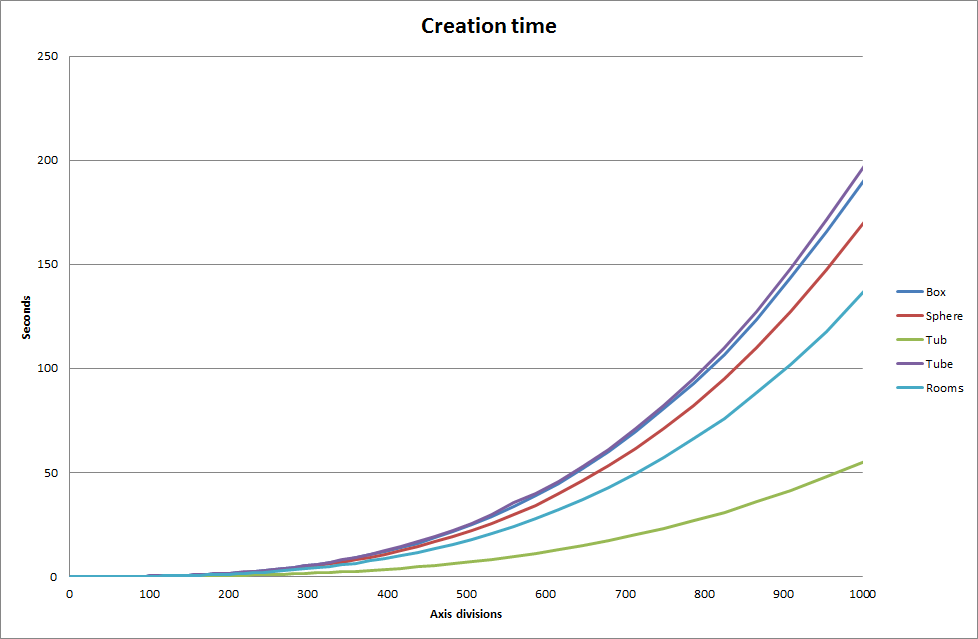
\includegraphics[width=\textwidth]{images/chart_voxel_creation_time}
    \caption{creation time} \label{fig:voxel creation time} \end{subfigure}
	\begin{subfigure}[h]{0.49\textwidth}
	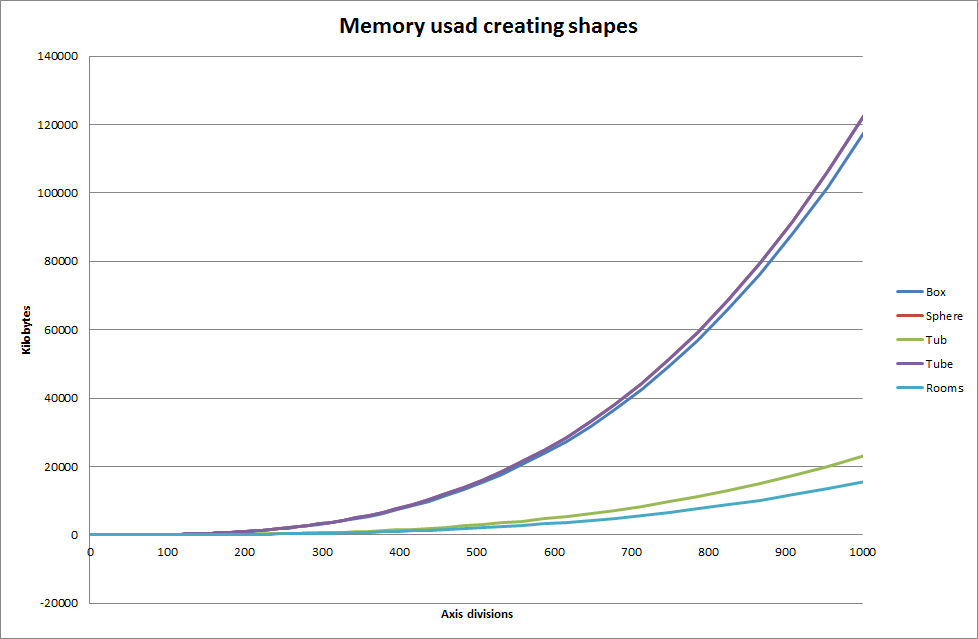
\includegraphics[width=\textwidth]{images/chart_voxel_creation_memory}
	\caption{memory} \label{fig:voxel memory} \end{subfigure}
    \caption{Voxel benchmark charts}\label{fig:voxel benchmark charts}
\end{figure}

For the voxel grid the results depends on how coarsely the grid is subdivided. Line graphs are shown to visualise this relationship. The number of division on the longest axis of the shape is used for the x axis. However the grids do not necessarily have the same dimensions on the other axis since the shapes are not square. For example for Axis divisions 200 the grid has the following resolution:
\begin{table}[htbp]
  \centering
  \caption{Example of voxel grid resolutions}
    \begin{tabular}{rr}
    \toprule
    Shape & Grid resolution \\
    \midrule
    Box   & 199x193x200 \\
    Sphere & 200x200x200 \\
    Tub   & 200x50x150 \\
    Tube  & 200x200x200 \\
    Rooms & 200x40x128 \\
    \bottomrule
    \end{tabular}%
  \label{tab:addlabel}%
\end{table}%



\subsubsection{Error}
The figure \ref{fig:voxel error} shows that the Rooms shape error oscillate as the number of divisions increase. At the lowest divisions all errors are high. The graph is clamped at 100\% but the Box and Rooms shapes have errors over 100\%. The trend for all shapes are that the error decreases as the number of divisions increase.

Figure \ref{fig:voxel error zoomed} zoomed in, showing only axis division up to 100. The figure shows that the Box and Sphere shapes don’t oscillate but the others do. We can also see that the Tube shape oscillate a little but not as much as the Tub and Rooms.

Looking at the numbers in appendix \ref{tab:Voxel Error} we see that the Sphere shape reaches 1\% error at around 75 divisions while box Box and Tube reaches 1\% error at around 110 divisions. The Tub oscillate around 1\% at roughly 250 division. The Rooms shape has some minimums below 1\%, but stabilizes at 2\% after 900 divisions.

\subsubsection{Running time}
Figure \ref{fig:voxel running time}) shows that the running time for the different shapes are close to linear to the number axis divisions. The Tub and Rooms have lower running time because there are less division in the other axis.

\subsubsection{Creation time}
Figure \ref{fig:voxel creation time} show how long it took to generate the voxel grid. The cells were populated by sampling the middle of the cell and using the boolean representation to find out if the position was inside shape. The creation time is dependent on the number of cells in grid and the complexity of the boolean representation. For example the Rooms shape has less cells than the corresponding Tub, but takes longer to create because the boolean model is more complex. However all shapes have exponential creation time.

\subsubsection{Memory used creating shapes}
Figure \ref{fig:voxel memory} show that the memory used creating the shape corresponds to the number of cells in the grid.

\subsection{Mesh triangulation}
\begin{figure}[h] \centering 
	\begin{subfigure}[h]{0.49\textwidth} 
	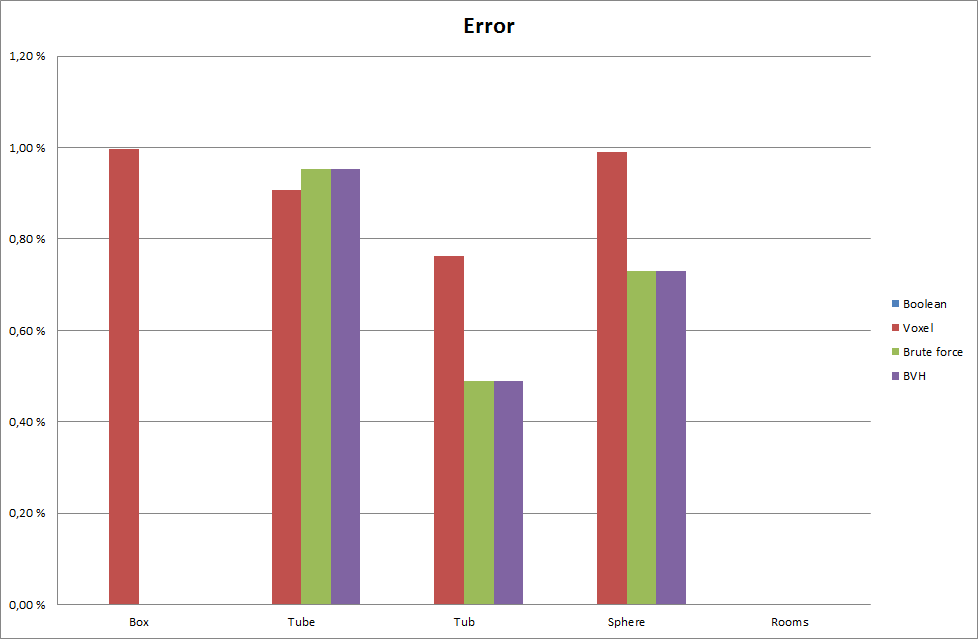
\includegraphics[width=\textwidth]{images/chart_comparison_error}
	\caption{error} \label{fig:comparison_error} \end{subfigure}
    \begin{subfigure}[h]{0.49\textwidth}
	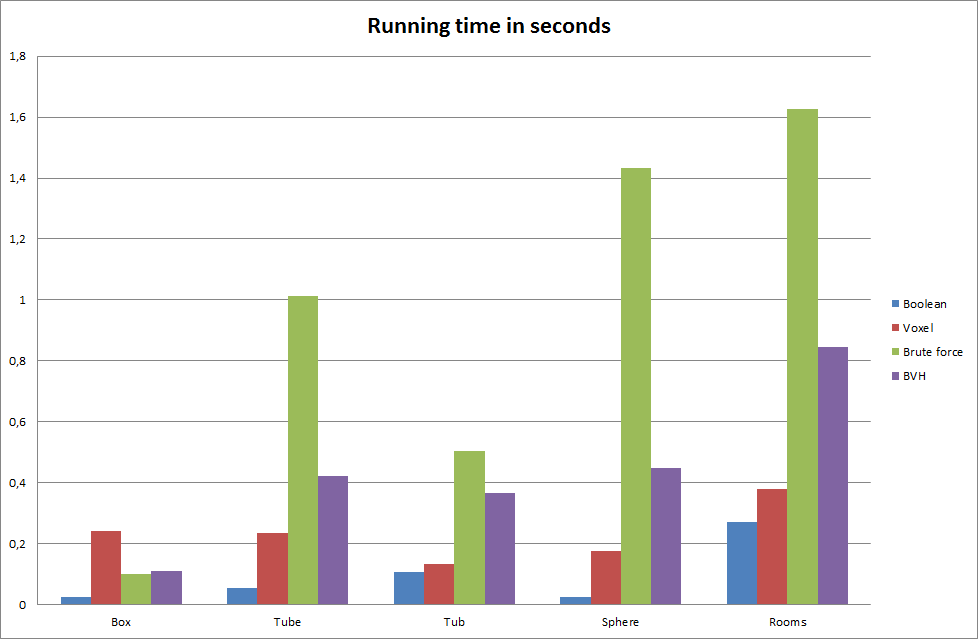
\includegraphics[width=\textwidth]{images/chart_comparison_running_time}
    \caption{running time} \label{fig:comparison_running_time} \end{subfigure}
    \begin{subfigure}[h]{0.49\textwidth}
	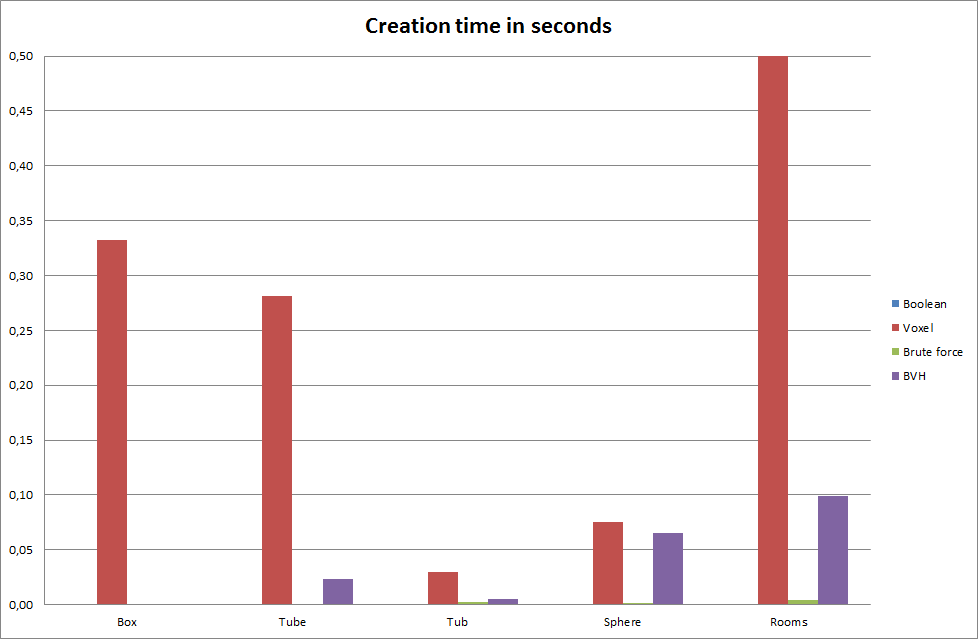
\includegraphics[width=\textwidth]{images/chart_comparison_creation_time}
    \caption{creation time} \label{fig:comparison_creation_time} \end{subfigure}
	\begin{subfigure}[h]{0.49\textwidth}
	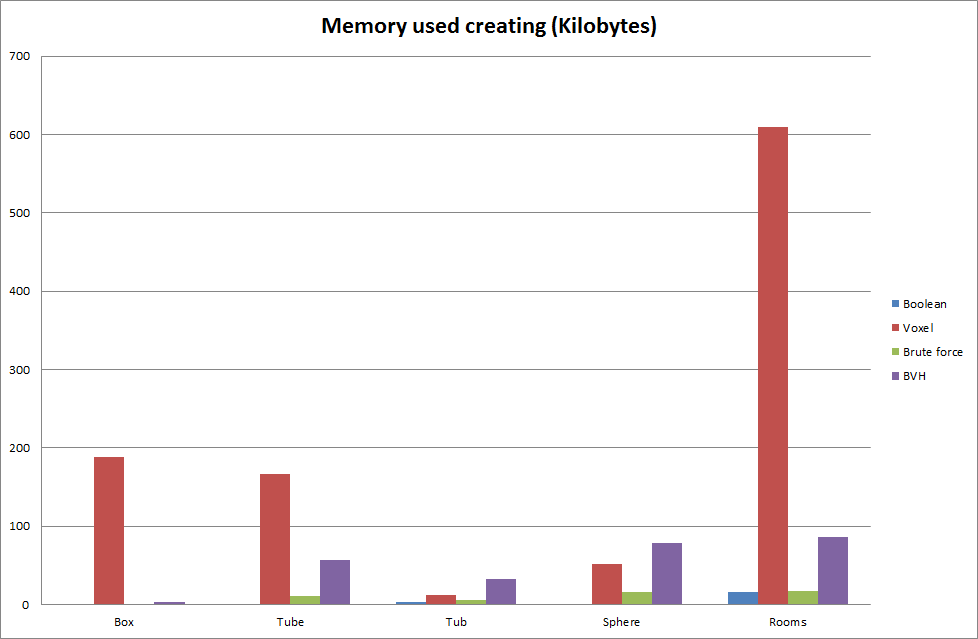
\includegraphics[width=\textwidth]{images/chart_comparison_creation_memory}
	\caption{memory} \label{fig:comparison_creation_memory} \end{subfigure}
    \caption{Comparison charts}\label{fig:comparison}
\end{figure}

For the mesh triangulated shapes the results depends on how many triangles there are in the mesh. The results are visualised in the graphs in figure \ref{fig:triangulate benchmark charts}. For the sphere and tube shapes we were able to generate shapes with a varying number of triangles. These are represented as lines in the chart. The other shapes only have one resolution and are represented as points in the chart. The tub and rooms shapes were hand modelled so have only one resolution. For the box shape it made no sense to tessellate as it would not increase the accuracy.

\subsubsection{Error}
The error chart in figure \ref{fig:sphere error} show that the box and rooms shapes have an error close to zero. Here the mesh triangulation is able to match the boolean representation almost perfectly. The error is most likely due to floating point rounding errors in the calculations. The tub shape is modelled with 100 triangles and have an error of 0.5\%. The Tub shape have some rounded areas that the triangles do not fit perfectly.

For the tube and sphere shapes we see that the error decreases as the number of triangles increase. For the sphere the version with radius adjusted to preserve volume is much better than the one with constant radius. The adjusted sphere reaches 1\% error at around 200 triangles while the constant radius sphere reaches the same after over 1000 triangles.

For the tube shape the error is higher then the adjusted sphere up until around 190 triangles. After that the error is lower. The tube shape is generated using a constant radius. This makes it less accurate in preserving the volume and has higher error. However the shape is less round than the sphere. It only has to be subdivided around one axis. So using more triangles have greater effect than on the sphere with constant radius.

The error for the BVH and brute force versions are identical. Only one of the results are shown reduce clutter.

\subsubsection{Running time}
The running time chart in figure \ref{fig:sphere running time} show that there is a big difference between the brute force and the BVH algorithms. With the brute force algorithm the time increase linearly with the number of triangles. The running time is logarithmic for the bounding volume hierarchy (BVH) method. 

The error for the Tube shape is slightly higher than for the sphere. Also the error for the Rooms shape is much higher than the tube and spheres with roughly the same number of triangles. This can be explained by them having a mesh structure which generates a less ideal BVH tree. The rooms shape in particular have large triangles which creates less optimal trees.

Even though the BVH scales much better it is slower when there are very few triangles. Up to around 40-50 triangles the brute force method is faster. This is likely due to the BVH algorithm having a higher overhead. Also the triangles will be relatively large compared to each other, creating an less optimal tree.

For the sphere the version with adjusted and constant radius game almost the same results. The sphere with adjusted radius was not included in the graph for clarity.

\subsubsection{Creation time}
The chart in figure \ref{fig:sphere creation time} shows that the BVH algorithm has an exponential creation time. It is difficult from the graph to see how the brute force complexity grows, but it is very low.

\subsubsection{Memory used to create shapes}
Figure \ref{fig:sphere creation memory} shows the memory used after creating the different shapes. The BVH implementations uses more memory than the brute force versions. The tub and and rooms shapes is on the tube line. Meaning they use about the same memory as the generated shapes with the comparable triangle counts. Compared to their BVH versions the brute force implementations use significantly less memory. The sphere brute force on the other hand only uses slightly less memory than its BVH implementation. It is unknown why this is. From the charts it seems that both brute force and BVH has linear complexity for all shapes.

\section{Comparing algorithms}

Figure \ref{fig:comparison} compares the different algorithms. Brute force and BVH are the two triangle mesh algorithms. For the procedural shapes sphere and tube the triangulation which gives an error that is less than 1\% was chosen.

\subsection{Error}
The running time chart in figure \ref{fig:comparison_error} shows that all algorithms managed to represent the shapes with less than 1\% error. 

\subsection{Running time}
The chart in figure \ref{fig:comparison_running_time} shows that Boolean is the fastest method followed by Voxels. Then comes bounding volume hierarchy (BVH) and brute force mesh. The exception is the rotated box shape where the rotation requires that a high number of voxels are generated to have less than 1\% error. Here the voxel is the slowest method. Also the box mesh is so simple that the benefit of the BVH is lost and it is in fact slightly slower than brute force.

The chart shows that the benefit of the BVH representation increases with the number of triangles. But it also shows that benfit of the BVH depends on the layout of the triangles. The sphere shape has an ideal layout with equally sized triangles spread evenly. This is shown by the big difference between the BVH and brute force. The tub and rooms shapes have large triangles that cover large areas of the shapes, reducing the benefit of the BVH tree. So the difference in running time is less for these shapes.

\subsection{Creation time}
Creating the voxel takes to most time. This time is spent populating the 3 dimensional grid. Creating the BVH trees is also slow. Mainly because it uses a brute force $O(n^3)$ algorithm for creating the tree. Boolean and brute force takes very little time to create.

\subsection{Memory used creating shapes}
The memory used to create the shapes using the different methods are shown in figure \ref{fig:comparison_creation_memory}. It shows that the voxel method used the most memory followed by BVH. The other methods have very low memory usage. However measuring memory is not exact and must be interpreted with caution. 

\begin{figure}[h] \centering 
	\begin{subfigure}[h]{0.49\textwidth}
	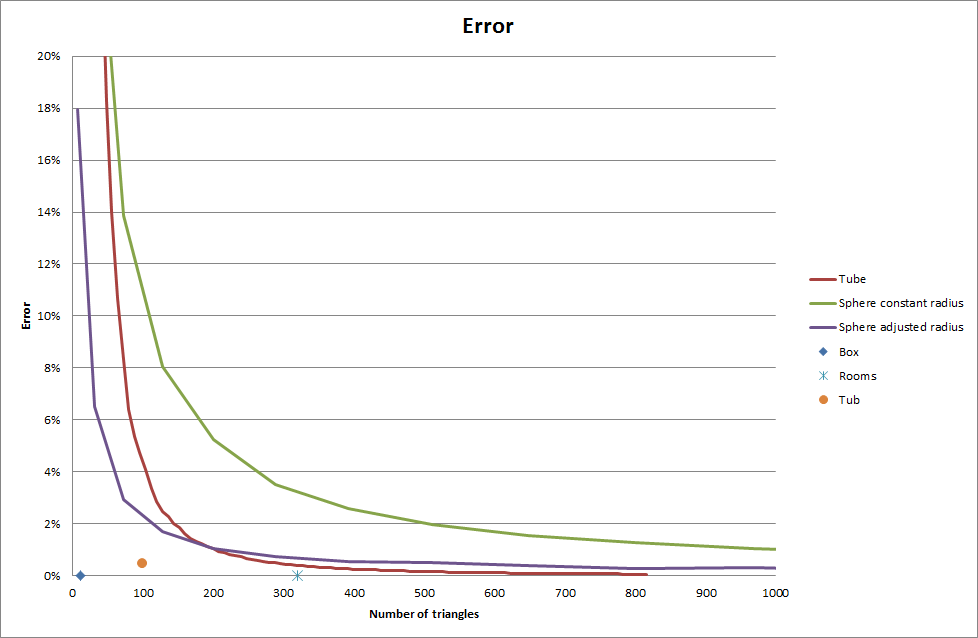
\includegraphics[width=\textwidth]{images/chart_triangulation_error}
	\caption{error} \label{fig:sphere error} \end{subfigure}
    \begin{subfigure}[h]{0.49\textwidth}
	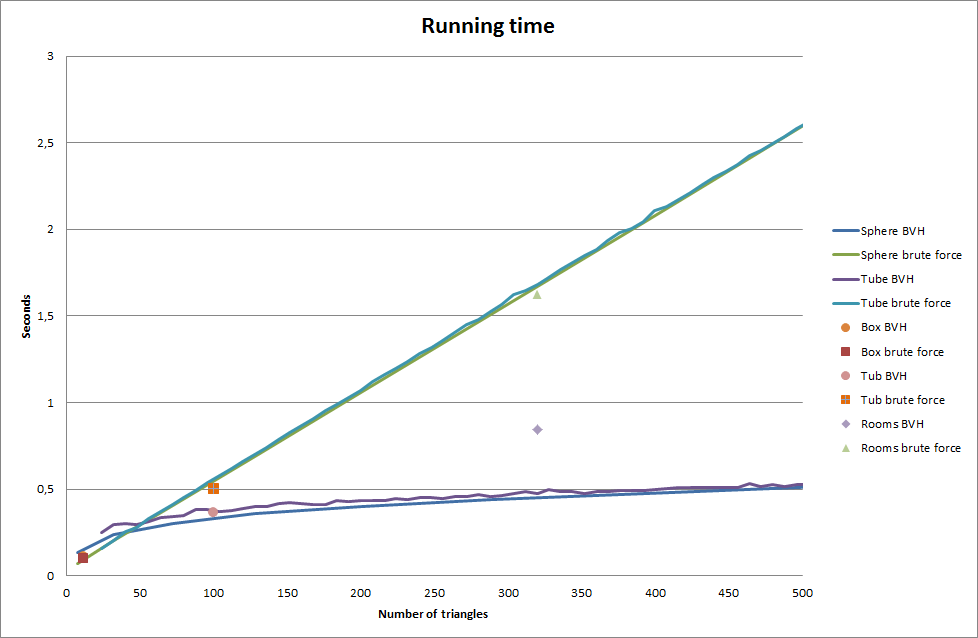
\includegraphics[width=\textwidth]{images/chart_triangulation_running_time}
    \caption{running time} \label{fig:sphere running time} \end{subfigure}
    \begin{subfigure}[h]{0.49\textwidth}
	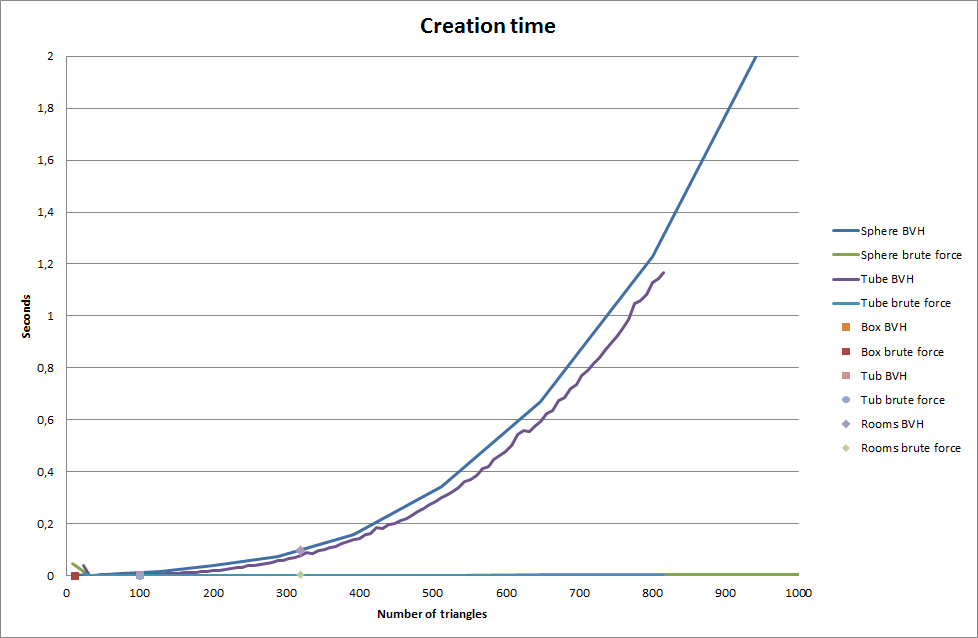
\includegraphics[width=\textwidth]{images/chart_triangulation_creation_time}
    \caption{creation time} \label{fig:sphere creation time} \end{subfigure}
	\begin{subfigure}[h]{0.49\textwidth} 
	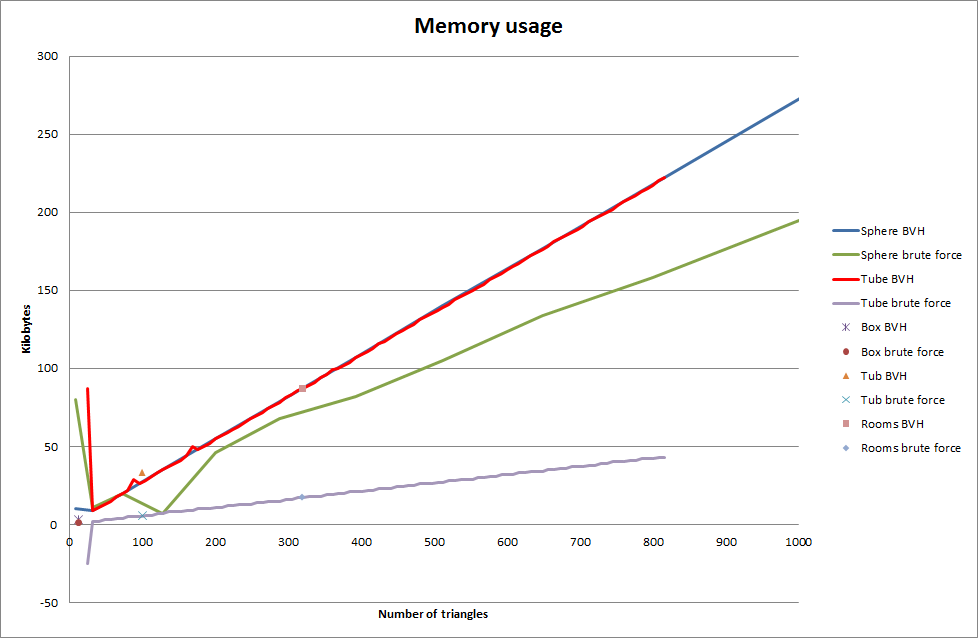
\includegraphics[width=\textwidth]{images/chart_triangulation_memory}
	\caption{memory} \label{fig:sphere creation memory} \end{subfigure}
    \caption{Mesh triangulation charts}\label{fig:triangulate benchmark charts}
\end{figure}

\chapter{Discussion}
\label{chapter:Discussion and Future Research}
In this chapter we review the algorithms with regards to the research questions. Future research that can improve the calculation of complex shielding is discussed in section \ref{section:Future Research}

\section{Discussion}

\section{Future Research}
\label{section:Future Research}

-other algorithms
-improving algorithms presented in this thesis
-more elaborate testing / benchmarking.
-method: how the measure accuracy
\subsection{Boolean}
The implementation used in this thesis evaluates all nodes in the boolean tree. This can be inefficient if there are many nodes. It would be possible to do culling on the internal nodes. If none of the children are intersected then the result of a unite or subtract operation will still be empty. However the boolean tree is not structured to be an efficient way of subdividing the space so the benefit may be limited. There might be possible to restructure the boolean tree that makes the culling more efficient while preserving the logical correctness. For example the result of uniting a set of objects is independent on the order and could be a subject for optimisation.

\subsection{Voxel}
The main issue with using a regular grid of voxels is the memory consumption. There are more efficient ways of representing the voxel grid. For example by using a sparse voxel octree \cite{laine2011efficient}. The octree will reduce the memory used by efficiently encoding empty regions of space. The algorithm is also possible to implement and run on the GPU for increased performance. The High Resolution Sparse Voxel DAGs \cite{kampe2013high} paper shows that a binary voxel grid can be represented orders of magnitude more efficently than using a sparse voxel octree by generalising the tree to a directed acyclic graph (DAG). The DAG is allows for efficient encoding of identical regions of space, as nodes are allowed to share pointers to identical subtrees. Implementing an algorithm that uses a hierarchical representation would alleviate the memory problem and allow for much higher grid resolutions. This can be very promising way to represent a complex shield and is a prime subject for future research.

\subsection{Triangles}
-alternative to BVH, efficent BVH building algorithm \cite{gu2013efficient}.



\chapter{Conclusion}
\label{chapter:Conclusion}
This thesis have investigated methods for calculating intersection with complex shields to be used with the point-kernel dose calculations. Three methods were selected for closer inspection and were analysed and benchmarked.

The boolean algorithm with primitives gave the best results in the benchmarks. It also fares well in the algorithm analysis, where only the BVH has better average case complexity. If the shape can be represented using boolean primitives then this will give the best results performance wise. This includes accuracy, running time and memory usage. The boolean algorithm can not only be used with primitives but any algorithm that returns a sorted list of non overlapping intersection segments. This makes it a valuable part in any method for creating complex shielding. One could for example create a shield consisting of a voxel shape subtracted from a triangle mesh.

The triangle mesh using BVH has the best average case running time complexity of $O(log n)$. However the number of triangles needed to represent certain shapes can be quite high. In the benchmarks the BVH is slower than boolean and voxel representation. The shapes have to be a lot more complex than the ones used in this thesis before the benefit of the logarithmic running time beats the other algorithms. The brute force algorithm were by far the slowest method and can not recommended. 

The voxel algorithm is fast and in some cases close to the boolean algorithm in the benchmarks. But the $O(n^3)$ memory usage severely limits the size of the grid which limits the types of shapes that can be represented with enough accuracy. Voxels are a viable options but are not a fully general solution given this limitations. Implementing a hierarchical voxel algorithm like sparse voxel octree would probably solve this problem making voxels a good candidate for representing complex shields.

\bibliographystyle{plain}
\bibliography{master}

\listoffigures
\listoftables
\appendix
\chapter{Source Code}

\section{Find timer resolution}
\label{source:timer_timer_resolution}
\begin{lstlisting}
private static void findTimerResolution() {
    long[] times = new long[100];
    for (int i=0; i<100; i++) {
        times[i] = System.nanoTime();
    }
    for (int i=1; i<100; i++) {
        long dif = times[i] - times[i - 1];
        if (dif != 0) {
            System.out.println(dif);
        }
    }
}
\end{lstlisting}

\section{Boolean unite}
\label{source:unite}
\begin{lstlisting}
public static Segments unite(Segments[] segmentsList, Segments out) {
    out.segmentCount = 0;
    int[] indexes = new int[segmentsList.length];
    while (true) {
        Segments minSeg = null;
        int segmentIndex = -1;
        int minIdx = -1;
        float minFrom = Float.NaN;
        for (int i=0; i<indexes.length; i++) {
            Segments s = segmentsList[i];
            int index = indexes[i];
            if (index < s.segmentCount) {
                if (Float.isNaN(minFrom) || s.from(index) < minFrom) {
                    minSeg = s;
                    minIdx = index;
                    minFrom = s.from(minIdx);
                    segmentIndex = i;
                }
            }
        }
        if (minIdx == -1) {
            break;
        }
        indexes[segmentIndex]++;

        if (out.segmentCount <= 0) {
            out.addAtEnd(minSeg.from(minIdx), minSeg.to(minIdx));
        } else {
            if (minSeg.from(minIdx) > out.to(out.segmentCount-1)) {
                // after end of out
                out.addAtEnd(minSeg.from(minIdx), minSeg.to(minIdx));
            } else {
                // overlap
                if (minSeg.to(minIdx) > out.to(out.segmentCount-1)) {
                    // new segment is higher than current
                    out.setTo(out.segmentCount-1, minSeg.to(minIdx));
                }
            }
        }
    }

    return out;
}
\end{lstlisting}

\section{Boolean subtract}
\label{source:unite}
\begin{lstlisting}
/**
 * out = a - b
 */
public static Segments subtract(Segments a, Segments b, Segments out) {
    out.segmentCount = 0;
    int aIdx = 0;
    int bIdx = 0;

    while (aIdx < a.segmentCount && bIdx < b.segmentCount) {
        if (b.to(bIdx) < a.from(aIdx)) {
            // b is before a
            bIdx++;
            continue;
        }
        if (b.from(bIdx) > a.to(aIdx)) {
            // b is after a
            out.addAtEnd(a.from(aIdx), a.to(aIdx));
            aIdx++;
            continue;
        }

        out.addAtEnd(a.from(aIdx), a.to(aIdx));
        aIdx++;

        // while b is inside last in out
        while (bIdx < b.segmentCount 
        		&& b.from(bIdx) < out.to(out.segmentCount-1)) {
            if (b.from(bIdx) < out.from(out.segmentCount-1)) {
                // b starts before out
                if (b.to(bIdx) > out.to(out.segmentCount-1)) {
                    // .. and ends after out: remove out
                    out.segmentCount--;
                    break;
                }
                // .. and ends before out
                out.setFrom(out.segmentCount-1, b.to(bIdx));
                bIdx++;
            } else {
                // b starts after out
                if (b.to(bIdx) > out.to(out.segmentCount-1)) {
                    // .. and ends after out
                    out.setTo(out.segmentCount-1, b.from(bIdx));
                    break;
                } else {
                    // ..and ends before out (inside out)
                    float outTo = out.to(out.segmentCount-1);
                    out.setTo(out.segmentCount-1, b.from(bIdx));
                    out.addAtEnd(b.to(bIdx), outTo);
                    bIdx++;
                }
            }
        }
    }

    while (aIdx < a.segmentCount) {
        out.addAtEnd(a.from(aIdx), a.to(aIdx));
        aIdx++;
    }

    return out;
}
\end{lstlisting}


\section{Voxel Grid Raytrcing}
\label{source:Voxel_Grid_Raytrace}
\begin{lstlisting} 
package trb.complexshield.voxel;

public class Raytrace {
    private VoxelGrid voxelGrid;
    private int x;
    private int y;
    private int z;
    private float dtDx;
    private float dtDy;
    private float dtDz;
    private float t;
    private int n;
    private int xInc;
    private int yInc;
    private int zInc;
    private float tNextY;
    private float tNextX;
    private float tNextZ;

    public Raytrace(VoxelGrid voxelGrid) {
        this.voxelGrid = voxelGrid;
    }

    public void raytrace(Line line, Output output) {
        initVariables(line);
        boolean wasInside = voxelGrid.getBitAtIndex(x, y, z);
        float wasT = 0f;
        while (true) {
            output.addIntersection(line, x, y, z, t);
            step();
            if (t > 1) {
                break;
            }
            boolean isInside = voxelGrid.getBitAtIndex(x, y, z);
            if (isInside != wasInside) {
                if (!isInside) {
                    output.addSegment(line, wasT, t);
                }

                wasT = t;
                wasInside = isInside;
            }
        }
        if (wasT < 1) {
            output.addIntersection(line, x, y, z, 1f);
        }
        if (wasInside && wasT < 1) {
            output.addSegment(line, wasT, 1);
        }
    }

    private void initVariables(Line line) {
        float x1 = line.p1.x;
        float x2 = line.p2.x;
        float y1 = line.p1.y;
        float y2 = line.p2.y;
        float z1 = line.p1.z;
        float z2 = line.p2.z;
        float dx = Math.abs(x2 - x1);
        float dy = Math.abs(y2 - y1);
        float dz = Math.abs(z2 - z1);

        x = (int) floor(x1);
        y = (int) floor(y1);
        z = (int) floor(z1);


        dtDx = 1f / dx;
        dtDy = 1f / dy;
        dtDz = 1f / dz;

        if (dx == 0) {
            xInc = 0;
            tNextX = dtDx; // infinity
        } else if (x2 > x1) {
            xInc = 1;
            n += ((int) floor(x2)) - x;
            tNextX = (floor(x1) + 1 - x1) * dtDx;
        } else {
            xInc = -1;
            n += x - (int) floor(x2);
            tNextX = (x1 - floor(x1)) * dtDx;
        }

        if (dy == 0) {
            yInc = 0;
            tNextY = dtDy; // infinity
        } else if (y2 > y1) {
            yInc = 1;
            n += (int) floor(y2) - y;
            tNextY = (floor(y1) + 1 - y1) * dtDy;
        } else {
            yInc = -1;
            n += y - (int) floor(y2);
            tNextY = (y1 - floor(y1)) * dtDy;
        }

        if (dz == 0) {
            zInc = 0;
            tNextZ = dtDz; // infinity
        } else if (z2 > z1) {
            zInc = 1;
            n += (int) floor(z2) - z;
            tNextZ = (floor(z1) + 1 - z1) * dtDz;
        } else {
            zInc = -1;
            n += z - (int) floor(z2);
            tNextZ = (z1 - floor(z1)) * dtDz;
        }
    }

    private float floor(float value) {
        return (float) Math.floor(value);
    }

    private void step() {
        if (tNextY < tNextX) {
            if (tNextZ < tNextY) {
                z += zInc;
                t = tNextZ;
                tNextZ += dtDz;
            } else {
                y += yInc;
                t = tNextY;
                tNextY += dtDy;
            }
        } else if (tNextZ < tNextX) {
            z += zInc;
            t = tNextZ;
            tNextZ += dtDz;
        } else {
            x += xInc;
            t = tNextX;
            tNextX += dtDx;
        }
    }

    public interface Output {
        void addIntersection(Line line, int x, int y, int z, float t);

        void addSegment(Line line, float wasT, float t);
    }
}
\end{lstlisting}

\chapter{Benchmark Data}
\section{Voxel Error}
	{\footnotesize
    \begin{longtable}{rrrrrr}
    \toprule
    dim   & Box   & Sphere & Tub   & Tube  & Rooms \\
    \midrule
    1     & 286,42 \% & 67,28 \% & 100,00 \% & 100,00 \% & 100,00 \% \\
    2     & 97,16 \% & 67,28 \% & 100,00 \% & 63,63 \% & 387,99 \% \\
    3     & 42,32 \% & 33,05 \% & 82,08 \% & 40,27 \% & 173,62 \% \\
    4     & 37,85 \% & 19,90 \% & 86,80 \% & 22,95 \% & 100,00 \% \\
    5     & 24,71 \% & 20,81 \% & 42,26 \% & 16,98 \% & 113,57 \% \\
    6     & 21,73 \% & 18,01 \% & 28,11 \% & 29,25 \% & 133,76 \% \\
    7     & 18,60 \% & 12,00 \% & 20,72 \% & 12,39 \% & 87,79 \% \\
    8     & 15,55 \% & 9,80 \% & 18,14 \% & 9,79 \% & 100,00 \% \\
    9     & 14,66 \% & 9,14 \% & 29,52 \% & 15,84 \% & 84,02 \% \\
    10    & 12,37 \% & 8,85 \% & 31,50 \% & 12,80 \% & 83,05 \% \\
    11    & 11,32 \% & 7,86 \% & 35,27 \% & 9,23 \% & 77,36 \% \\
    12    & 10,47 \% & 6,64 \% & 37,26 \% & 9,35 \% & 100,00 \% \\
    13    & 9,53 \% & 6,65 \% & 24,48 \% & 8,33 \% & 75,88 \% \\
    14    & 8,95 \% & 6,06 \% & 19,88 \% & 10,61 \% & 73,35 \% \\
    15    & 8,23 \% & 5,29 \% & 16,53 \% & 6,20 \% & 78,43 \% \\
    16    & 7,69 \% & 5,18 \% & 15,98 \% & 5,42 \% & 100,00 \% \\
    17    & 7,32 \% & 4,67 \% & 17,91 \% & 7,53 \% & 81,08 \% \\
    18    & 6,81 \% & 4,43 \% & 20,56 \% & 6,38 \% & 72,13 \% \\
    19    & 6,57 \% & 4,51 \% & 22,62 \% & 5,45 \% & 80,78 \% \\
    20    & 6,10 \% & 3,95 \% & 23,05 \% & 4,93 \% & 100,00 \% \\
    21    & 5,83 \% & 3,84 \% & 21,10 \% & 4,86 \% & 71,09 \% \\
    22    & 5,53 \% & 3,51 \% & 17,59 \% & 5,61 \% & 76,31 \% \\
    23    & 5,22 \% & 3,48 \% & 14,58 \% & 4,40 \% & 81,92 \% \\
    24    & 5,08 \% & 3,38 \% & 14,08 \% & 4,18 \% & 70,38 \% \\
    25    & 4,82 \% & 3,04 \% & 11,36 \% & 4,07 \% & 69,31 \% \\
    26    & 4,64 \% & 3,07 \% & 13,52 \% & 5,22 \% & 74,67 \% \\
    27    & 4,47 \% & 2,92 \% & 14,92 \% & 3,56 \% & 84,28 \% \\
    28    & 4,36 \% & 2,70 \% & 15,08 \% & 3,50 \% & 100,00 \% \\
    29    & 4,16 \% & 2,75 \% & 11,11 \% & 3,71 \% & 65,41 \% \\
    30    & 4,03 \% & 2,69 \% & 8,49 \% & 3,87 \% & 77,07 \% \\
    32    & 3,75 \% & 2,38 \% & 5,86 \% & 3,08 \% & 70,51 \% \\
    34    & 3,55 \% & 2,26 \% & 6,73 \% & 3,72 \% & 77,98 \% \\
    36    & 3,37 \% & 2,11 \% & 8,61 \% & 2,42 \% & 100,00 \% \\
    38    & 3,19 \% & 2,07 \% & 3,27 \% & 3,02 \% & 79,89 \% \\
    40    & 3,00 \% & 1,92 \% & 1,24 \% & 2,44 \% & 71,23 \% \\
    42    & 2,82 \% & 1,79 \% & 5,74 \% & 3,06 \% & 58,32 \% \\
    44    & 2,69 \% & 1,74 \% & 7,68 \% & 2,23 \% & 55,17 \% \\
    46    & 2,60 \% & 1,66 \% & 4,68 \% & 2,49 \% & 49,12 \% \\
    48    & 2,48 \% & 1,58 \% & 3,37 \% & 2,16 \% & 52,25 \% \\
    50    & 2,38 \% & 1,52 \% & 7,40 \% & 2,24 \% & 59,83 \% \\
    53    & 2,24 \% & 1,42 \% & 7,39 \% & 1,88 \% & 53,82 \% \\
    56    & 2,12 \% & 1,34 \% & 4,99 \% & 1,72 \% & 31,22 \% \\
    59    & 2,01 \% & 1,26 \% & 8,37 \% & 1,73 \% & 30,22 \% \\
    62    & 1,90 \% & 1,20 \% & 6,36 \% & 1,93 \% & 24,96 \% \\
    65    & 1,81 \% & 1,14 \% & 4,58 \% & 1,63 \% & 30,63 \% \\
    68    & 1,73 \% & 1,11 \% & 6,50 \% & 1,44 \% & 18,54 \% \\
    71    & 1,66 \% & 1,07 \% & 2,58 \% & 1,45 \% & 13,26 \% \\
    75    & 1,57 \% & 0,99 \% & 3,72 \% & 1,33 \% & 12,97 \% \\
    79    & 1,49 \% & 0,94 \% & 0,76 \% & 1,28 \% & 9,96 \% \\
    83    & 1,42 \% & 0,88 \% & 3,71 \% & 1,16 \% & 9,28 \% \\
    87    & 1,35 \% & 0,85 \% & 1,92 \% & 1,10 \% & 10,26 \% \\
    91    & 1,29 \% & 0,82 \% & 4,68 \% & 1,12 \% & 11,49 \% \\
    96    & 1,21 \% & 0,76 \% & 2,92 \% & 1,04 \% & 12,48 \% \\
    101   & 1,16 \% & 0,73 \% & 4,68 \% & 1,01 \% & 19,61 \% \\
    106   & 1,10 \% & 0,69 \% & 3,20 \% & 1,05 \% & 17,64 \% \\
    111   & 1,05 \% & 0,66 \% & 1,47 \% & 0,91 \% & 20,38 \% \\
    117   & 1,00 \% & 0,63 \% & 1,68 \% & 0,89 \% & 21,26 \% \\
    123   & 0,94 \% & 0,59 \% & 2,58 \% & 0,80 \% & 26,40 \% \\
    129   & 0,90 \% & 0,57 \% & 2,12 \% & 0,84 \% & 19,20 \% \\
    135   & 0,86 \% & 0,54 \% & 2,09 \% & 0,73 \% & 23,04 \% \\
    142   & 0,82 \% & 0,52 \% & 2,59 \% & 0,79 \% & 17,87 \% \\
    149   & 0,77 \% & 0,49 \% & 2,02 \% & 0,67 \% & 11,63 \% \\
    156   & 0,74 \% & 0,47 \% & 1,88 \% & 0,64 \% & 6,33 \% \\
    164   & 0,71 \% & 0,44 \% & 1,33 \% & 0,63 \% & 5,06 \% \\
    172   & 0,67 \% & 0,42 \% & 2,49 \% & 0,55 \% & 5,24 \% \\
    181   & 0,64 \% & 0,40 \% & 2,27 \% & 0,59 \% & 7,51 \% \\
    190   & 0,61 \% & 0,38 \% & 1,19 \% & 0,57 \% & 11,63 \% \\
    200   & 0,57 \% & 0,36 \% & 0,25 \% & 0,50 \% & 13,07 \% \\
    210   & 0,55 \% & 0,35 \% & 1,64 \% & 0,53 \% & 14,86 \% \\
    220   & 0,52 \% & 0,33 \% & 2,25 \% & 0,44 \% & 14,34 \% \\
    230   & 0,50 \% & 0,31 \% & 0,93 \% & 0,43 \% & 9,35 \% \\
    240   & 0,48 \% & 0,30 \% & 0,21 \% & 0,41 \% & 6,42 \% \\
    250   & 0,46 \% & 0,29 \% & 1,37 \% & 0,43 \% & 2,74 \% \\
    260   & 0,44 \% & 0,28 \% & 1,88 \% & 0,39 \% & 2,99 \% \\
    270   & 0,42 \% & 0,27 \% & 0,84 \% & 0,39 \% & 6,05 \% \\
    280   & 0,41 \% & 0,26 \% & 0,19 \% & 0,37 \% & 7,70 \% \\
    290   & 0,39 \% & 0,25 \% & 1,18 \% & 0,36 \% & 11,79 \% \\
    300   & 0,38 \% & 0,24 \% & 1,64 \% & 0,35 \% & 13,25 \% \\
    310   & 0,37 \% & 0,23 \% & 0,74 \% & 0,35 \% & 6,70 \% \\
    320   & 0,35 \% & 0,22 \% & 0,16 \% & 0,32 \% & 6,51 \% \\
    330   & 0,34 \% & 0,22 \% & 1,04 \% & 0,33 \% & 3,25 \% \\
    340   & 0,33 \% & 0,21 \% & 1,44 \% & 0,29 \% & 0,00 \% \\
    350   & 0,33 \% & 0,20 \% & 0,65 \% & 0,30 \% & 3,37 \% \\
    360   & 0,32 \% & 0,20 \% & 0,15 \% & 0,28 \% & 6,91 \% \\
    370   & 0,31 \% & 0,19 \% & 0,92 \% & 0,29 \% & 7,84 \% \\
    380   & 0,30 \% & 0,19 \% & 1,29 \% & 0,27 \% & 8,94 \% \\
    390   & 0,29 \% & 0,18 \% & 0,59 \% & 0,27 \% & 8,25 \% \\
    400   & 0,28 \% & 0,18 \% & 0,13 \% & 0,25 \% & 5,54 \% \\
    410   & 0,28 \% & 0,17 \% & 0,84 \% & 0,26 \% & 3,94 \% \\
    420   & 0,27 \% & 0,17 \% & 1,17 \% & 0,24 \% & 1,67 \% \\
    430   & 0,26 \% & 0,17 \% & 0,53 \% & 0,25 \% & 1,81 \% \\
    440   & 0,26 \% & 0,16 \% & 0,12 \% & 0,23 \% & 3,68 \% \\
    450   & 0,25 \% & 0,16 \% & 0,76 \% & 0,24 \% & 5,39 \% \\
    460   & 0,25 \% & 0,16 \% & 0,87 \% & 0,23 \% & 8,06 \% \\
    470   & 0,24 \% & 0,15 \% & 0,48 \% & 0,23 \% & 8,60 \% \\
    480   & 0,23 \% & 0,15 \% & 0,10 \% & 0,21 \% & 4,46 \% \\
    490   & 0,23 \% & 0,15 \% & 0,73 \% & 0,21 \% & 4,38 \% \\
    500   & 0,23 \% & 0,14 \% & 0,99 \% & 0,20 \% & 2,23 \% \\
    510   & 0,22 \% & 0,14 \% & 0,45 \% & 0,21 \% & 0,00 \% \\
    520   & 0,22 \% & 0,14 \% & 0,09 \% & 0,19 \% & 2,25 \% \\
    530   & 0,21 \% & 0,14 \% & 0,64 \% & 0,20 \% & 4,66 \% \\
    540   & 0,21 \% & 0,13 \% & 0,91 \% & 0,19 \% & 5,89 \% \\
    550   & 0,21 \% & 0,13 \% & 0,42 \% & 0,19 \% & 6,70 \% \\
    560   & 0,20 \% & 0,13 \% & 0,09 \% & 0,18 \% & 5,86 \% \\
    570   & 0,20 \% & 0,13 \% & 0,60 \% & 0,18 \% & 3,54 \% \\
    580   & 0,19 \% & 0,12 \% & 0,85 \% & 0,18 \% & 2,93 \% \\
    590   & 0,19 \% & 0,12 \% & 0,39 \% & 0,18 \% & 1,20 \% \\
    600   & 0,19 \% & 0,12 \% & 0,09 \% & 0,17 \% & 1,30 \% \\
    610   & 0,18 \% & 0,12 \% & 0,56 \% & 0,17 \% & 3,26 \% \\
    620   & 0,18 \% & 0,11 \% & 0,80 \% & 0,16 \% & 3,90 \% \\
    630   & 0,18 \% & 0,11 \% & 0,37 \% & 0,16 \% & 6,32 \% \\
    640   & 0,18 \% & 0,11 \% & 0,08 \% & 0,16 \% & 6,42 \% \\
    650   & 0,17 \% & 0,11 \% & 0,53 \% & 0,16 \% & 3,39 \% \\
    660   & 0,17 \% & 0,11 \% & 0,63 \% & 0,15 \% & 3,34 \% \\
    670   & 0,17 \% & 0,11 \% & 0,34 \% & 0,15 \% & 1,69 \% \\
    680   & 0,17 \% & 0,10 \% & 0,07 \% & 0,15 \% & 0,00 \% \\
    690   & 0,16 \% & 0,10 \% & 0,50 \% & 0,15 \% & 1,69 \% \\
    700   & 0,16 \% & 0,10 \% & 0,71 \% & 0,14 \% & 3,50 \% \\
    710   & 0,16 \% & 0,10 \% & 0,32 \% & 0,15 \% & 4,48 \% \\
    720   & 0,16 \% & 0,10 \% & 0,07 \% & 0,14 \% & 5,51 \% \\
    730   & 0,15 \% & 0,10 \% & 0,47 \% & 0,15 \% & 4,58 \% \\
    740   & 0,15 \% & 0,10 \% & 0,67 \% & 0,14 \% & 3,15 \% \\
    750   & 0,15 \% & 0,09 \% & 0,31 \% & 0,14 \% & 2,30 \% \\
    760   & 0,15 \% & 0,09 \% & 0,07 \% & 0,13 \% & 0,94 \% \\
    770   & 0,15 \% & 0,09 \% & 0,44 \% & 0,14 \% & 1,01 \% \\
    780   & 0,14 \% & 0,09 \% & 0,64 \% & 0,13 \% & 2,04 \% \\
    790   & 0,14 \% & 0,09 \% & 0,29 \% & 0,13 \% & 3,47 \% \\
    800   & 0,14 \% & 0,09 \% & 0,06 \% & 0,12 \% & 4,98 \% \\
    810   & 0,14 \% & 0,09 \% & 0,42 \% & 0,13 \% & 5,15 \% \\
    820   & 0,14 \% & 0,09 \% & 0,61 \% & 0,12 \% & 2,77 \% \\
    830   & 0,14 \% & 0,09 \% & 0,28 \% & 0,12 \% & 2,33 \% \\
    840   & 0,13 \% & 0,08 \% & 0,06 \% & 0,12 \% & 1,36 \% \\
    850   & 0,13 \% & 0,08 \% & 0,42 \% & 0,12 \% & 0,44 \% \\
    860   & 0,13 \% & 0,08 \% & 0,58 \% & 0,12 \% & 1,36 \% \\
    870   & 0,13 \% & 0,08 \% & 0,26 \% & 0,12 \% & 2,80 \% \\
    880   & 0,13 \% & 0,08 \% & 0,06 \% & 0,12 \% & 3,58 \% \\
    890   & 0,13 \% & 0,08 \% & 0,38 \% & 0,12 \% & 4,46 \% \\
    900   & 0,13 \% & 0,08 \% & 0,56 \% & 0,11 \% & 3,78 \% \\
    910   & 0,12 \% & 0,08 \% & 0,25 \% & 0,11 \% & 2,63 \% \\
    920   & 0,12 \% & 0,08 \% & 0,17 \% & 0,11 \% & 1,90 \% \\
    930   & 0,12 \% & 0,08 \% & 0,37 \% & 0,11 \% & 0,25 \% \\
    940   & 0,12 \% & 0,08 \% & 0,53 \% & 0,11 \% & 0,83 \% \\
    950   & 0,12 \% & 0,07 \% & 0,23 \% & 0,11 \% & 1,67 \% \\
    960   & 0,12 \% & 0,07 \% & 0,05 \% & 0,11 \% & 2,48 \% \\
    970   & 0,12 \% & 0,07 \% & 0,35 \% & 0,11 \% & 4,08 \% \\
    980   & 0,11 \% & 0,07 \% & 0,41 \% & 0,10 \% & 4,32 \% \\
    990   & 0,11 \% & 0,07 \% & 0,23 \% & 0,11 \% & 2,21 \% \\
    1000  & 0,11 \% & 0,07 \% & 0,05 \% & 0,10 \% & 2,28 \% \\
    1010  & 0,11 \% & 0,07 \% & 0,34 \% & 0,10 \% & 0,90 \% \\
    1020  & 0,11 \% & 0,07 \% & 0,49 \% & 0,10 \% & 0,00 \% \\
    \bottomrule
    \end{longtable}}%
  \label{tab:Voxel Error}%



\end{document}